%!TEX root = Main.tex
\documentclass[Main]{subfiles}

\begin{document}

\section{Design, implementation and test setup} % (fold)
\label{sec:design_implementation_test_setup}

	\subsection{System Description}
		The main functional blocks of the system are shown in Figure \ref{fig:sysDesc}. 
		CO$_2$ emission data is acquired from the FTP server by the Java application. 
		The Java application determines whether the emission is high or low and transmits the corresponding control message to the ZigBee LED device. 
		The Sequence Executor Tool is used by the Java application for managing the communication with the ZigBee LED device. 
		By specifying the address of the SmartAMM server, ZigBee gateway ID and ZigBee LED device ID, the Java application is able to communicate with the ZigBee LED device.  

		\begin{figure}[H]
		\centering
		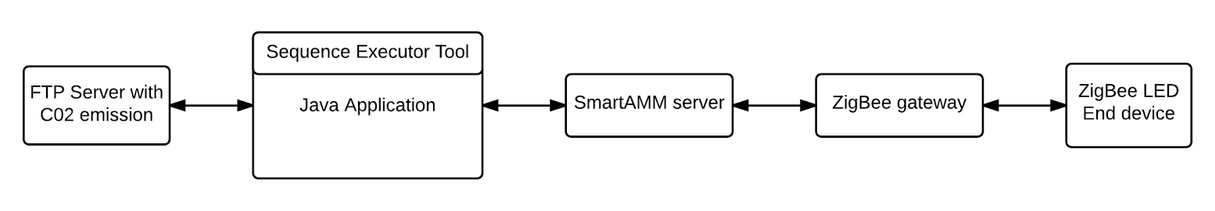
\includegraphics[width=\linewidth]{SystemDescription}
		\caption{System description}
		\label{fig:sysDesc}
		\end{figure}




	\subsection{Decision Making}


	\newpage
	\subsection{Sequence Executor Tool}
		The Sequence Executor Tool, which is provided by Develco Products, is a Java application able to communicate with ZigBee devices through a SmartAMM server.
		It requires two input files: A \emph{setting} file and a \emph{sequence} file.

		\subsubsection{Setting file}
			The \emph{settings} file is a XML file that contains various settings used in the tool. 
			The most relevant is settings regarding which server the tool should connect to. 
			In this project, the server was hosted on a local PC and the gateway was a USB dongle, which resulted in the following settings:
			\begin{itemize}
				\item gatewayType: ActiveMQ
				\item portNo: 62000
				\item hostName: localhost
			\end{itemize}

		\subsubsection{Sequence files}
			The \emph{sequence} file is also an XML file, specifying the sequence of telegrams to be sent to the ZigBee device, including gateway and device IDs. 
			It also specifies how to determine whether the telegram was successfully receive. 
			In this project positive acknowledgment are used as an indicator for successful transmission.
			In \ref{sec:appendix_a} the XML files for authorizing the ZigBee end device on the network, and setting the LED green is shown.
			Each sequence file contains the following items: 
			\begin{itemize}
				\item General sequence descriptions
				\item Substitute texts
				\item Steps
			\end{itemize}
			The general description contains information like sequence name, author, tool version etc.
			The substitute texts are a smart feature in the tool. 
			These allows the user to easily change certain fields in the steps. 
			A great example of this is the sequence file specifying setting the LED red or green.
			Instead of editing directly in the telegram defined in the step section, only the substitute texts need to be changed in order to set the LED red or green. 

			The last items in the sequence files are steps. 
			In both files shown in Appendix A there are two steps. 
			The first step in both files is used to connect to the gateway.
			The second step is used to transmit either an authorization telegram or a LED setting telegram.
			Each step contains a textual representation of the telegram to be transmitted, receive filters, an approval section and a general step description including a timeout interval.

			The receive filter is used to sort incoming telegrams, so that the correct telegram is used to verify the transmission status. 
			In the authorizing sequence, the receive filters sort for a device announce from the ZigBee device with the correct ID.
			
			The approval fields are used to validate the status of the telegram that gets through the receive filters. 
			In the Set LED Green sequence the received telegram must contain a \emph{Status} field with the value \emph{Success}.

			Given the sequence files, the tool is able to differentiate between \emph{Success}, \emph{Failure} and \emph{Timeout}.
			If no telegram passes through the receive filters within the timeout interval, the end status will be \emph{Timeout}.
			If a telegram passes through the receive filters but does not fulfill the approval fields, the end status will be \emph{Failure}.
			And if everything goes well, the end status is \emph{Success}.

		\subsubsection{Application interface}
			The Sequence Executor Tool is available as a .jar file, and can thus be included in a Java application, from which the main method of the Sequence Executor Tool can be called.


	\subsection{Application}



	\subsection{Communication Protocols}
		The system utilizes several different communication technologies.

		\subsection{FTP}
			File Transfer Protocol over TCP


		\subsection{SmartAMM}
			propreitær protokol udenom zigbee, wrapper protokol. SmartAMM protokol. 

		\subsection{ZigBee}
			As the LED device is ZigBee enabled, this is the technology of choice for communication. 
			ZigBee is a low power and low data rate wireless protocol for personal area networks. 
			The lower layers(MAC and PHY) of the protocol are based on the IEEE 802.15.4 standard\cite{ZigBeeSpec}, whereas higher layers such as network and application have been defined by the ZigBee Alliance.
			ZigBee features a range of different application profiles including Home Automation (HA), Building Automation, Light Link, Smart Energy etc\cite{ZigBeeApplicationProfiles:Online}.
			The LED device and gateway are both setup as HA devices. 

			\subsubsection{Commissioning}
				Commissioning   

			\subsubsection{Security}

			
			% subsection subsection_name (end)


		% Zigbee - Ivan Starter
		% Web protokoller - Ivan Starter
		% Det sidste



% section design_implementation_test_setup (end)
\end{document}